\documentclass{beamer}

% Beamer style
%\usetheme[secheader]{Madrid}
\usetheme{CambridgeUS}
\usecolortheme[rgb={0.65,0.15,0.25}]{structure}
%\usefonttheme[onlymath]{serif}
\beamertemplatenavigationsymbolsempty
%\AtBeginSubsection

% Packages
%\usepackage[french]{babel}
\usepackage[latin1]{inputenc}
\usepackage{color}
\usepackage{dsfont, stmaryrd}
\usepackage{amsmath, amsfonts, amssymb}
\usepackage{stmaryrd}
\usepackage{epsfig}
\usepackage{/media/donnees/LATEX/astats}
%\usepackage[all]{xy}
\usepackage{graphicx}

% Commands
\definecolor{darkred}{rgb}{0.65,0.15,0.25}
\definecolor{darkgreen}{rgb}{0,0.4,0}
\newcommand{\emphase}[1]{\textcolor{darkred}{#1}}
\newcommand{\paragraph}[1]{\emphase{#1}}
\newcommand{\refer}[1]{\textcolor{blue}{\sl \cite{#1}}}
\newcommand{\Refer}[1]{\textcolor{blue}{\sl #1}}
\newcommand{\newblock}{}

% Symbols
\newcommand{\Abf}{{\bf A}}
\newcommand{\Beta}{\text{B}}
\newcommand{\betabf}{\text{\mathversion{bold}{$\beta$}}}
\newcommand{\Bcal}{\mathcal{B}}
\newcommand{\BIC}{\text{BIC}}
\newcommand{\dd}{\text{d}}
\newcommand{\Cbf}{{\bf C}}
\newcommand{\dbf}{{\bf d}}
\newcommand{\Dcal}{\mathcal{D}}
\newcommand{\Esp}{\mathbb{E}}
\newcommand{\Ebf}{{\bf E}}
\newcommand{\Ecal}{\mathcal{E}}
\newcommand{\Gcal}{\mathcal{G}}
\newcommand{\Gam}{\mathcal{G}\text{am}}
\newcommand{\Ibb}{\mathbb{I}}
\newcommand{\Ibf}{{\bf I}}
\newcommand{\ICL}{\text{ICL}}
\newcommand{\Cov}{\mathbb{C}\text{ov}}
\newcommand{\Corr}{\mathbb{C}\text{orr}}
\newcommand{\Var}{\mathbb{V}}
\newcommand{\Vsf}{\mathsf{V}}
\newcommand{\pen}{\text{pen}}
\newcommand{\Fcal}{\mathcal{F}}
\newcommand{\Hbf}{{\bf H}}
\newcommand{\Hcal}{\mathcal{H}}
\newcommand{\Jcal}{\mathcal{J}}
\newcommand{\Kbf}{{\bf K}}
\newcommand{\Lcal}{\mathcal{L}}
\newcommand{\Lbf}{{\bf L}}
\newcommand{\Mcal}{\mathcal{M}}
\newcommand{\mbf}{{\bf m}}
\newcommand{\mum}{\mu(\mbf)}
\newcommand{\Ncal}{\mathcal{N}}
\newcommand{\Nbf}{{\bf N}}
\newcommand{\Nm}{N(\mbf)}
\newcommand{\Ocal}{\mathcal{O}}
\newcommand{\Obf}{{\bf 0}}
\newcommand{\Omegas}{\underset{s}{\Omega}}
\newcommand{\Pbf}{{\bf P}}
\newcommand{\Pcal}{\mathcal{P}}
\newcommand{\Qcal}{\mathcal{Q}}
\newcommand{\Rbb}{\mathbb{R}}
\newcommand{\Rcal}{\mathcal{R}}
\newcommand{\sbf}{{\bf s}}
\newcommand{\Sbf}{{\bf S}}
\newcommand{\Scal}{\mathcal{S}}
\newcommand{\Ucal}{\mathcal{U}}
\newcommand{\Vcal}{\mathcal{V}}
\newcommand{\Tbf}{{\bf T}}
\newcommand{\ubf}{{\bf u}}
\newcommand{\Ubf}{{\bf U}}
\newcommand{\Wbf}{{\bf W}}
\newcommand{\xbf}{{\bf x}}
\newcommand{\Xbf}{{\bf X}}
\newcommand{\Ybf}{{\bf Y}}
\newcommand{\Zbf}{{\bf Z}}
\newcommand{\pibf}{\text{\mathversion{bold}{$\pi$}}}
\newcommand{\Sigmabf}{\text{\mathversion{bold}{$\Sigma$}}}
\newcommand{\gammabf}{\text{\mathversion{bold}{$\gamma$}}}
\newcommand{\mubf}{\text{\mathversion{bold}{$\mu$}}}
\newcommand{\nubf}{\text{\mathversion{bold}{$\nu$}}}
\newcommand{\Thetabf}{\text{\mathversion{bold}{$\Theta$}}}
\newcommand{\thetabf}{\text{\mathversion{bold}{$\theta$}}}
\newcommand{\BP}{\text{BP}}
\newcommand{\EM}{\text{EM}}
\newcommand{\VEM}{\text{VEM}}
\newcommand{\VBEM}{\text{VB}}
\newcommand{\cst}{\text{cst}}
\newcommand{\obs}{\text{obs}}
\newcommand{\ra}{\emphase{$\rightarrow$~}}
\newcommand{\QZ}{Q_{\Zbf}}
\newcommand{\Qt}{Q_{\thetabf}}

% Directory
\newcommand{\fighd}{../Figures}
\newcommand{\figSimHMM}{../Figures/CGH-HMM-sim/CGHsim-9}


%====================================================================
\title[Segmentation and chromosomal alterations]{Segmentation methods
  for the detection of chromosomal alterations}

\author[S. Robin]{S. Robin}

\institute[AgroParisTech / INRA]{UMR 518 AgroParisTech / INRA Applied
  MAth \& Comput. Sc.\\
  \bigskip
  \begin{tabular}{ccccc}
    
\epsfig{file=../Figures/LogoINRA-Couleur.ps,
    width=2.5cm} & 
    \hspace{.5cm} &
    
\epsfig{file=../Figures/logagroptechsolo.eps,
    width=3.75cm} & 
    \hspace{.5cm} &
    
\epsfig{file=../Figures/logo-ssb.eps,
    width=2.5cm} \\ 
  \end{tabular} \\
  \bigskip
  }

  \date[Analyse du G�nome Tumoral]{Ecole Th�matique "Analyse du G�nome
    Tumoral" \\ Canc�rop�le IdF, Mafflier, March 2012}

%====================================================================

%====================================================================
%====================================================================
\begin{document}
%====================================================================
%====================================================================

%====================================================================
\frame{\titlepage
  }

%====================================================================
\frame{\frametitle{Outline} 
  \tableofcontents
  }

%====================================================================
%====================================================================
\section{Segmentation: The basic problem}
\frame{\frametitle{Segmentation: The basic problem}}
% ====================================================================
\frame{ \frametitle{Copy number variations in cancer cells} 
  Genomic alterations are associated with (responsible for?) various
  types of cancers.
  
  \begin{tabular}{cc}
    \onslide+<1->{Normal cell} & \onslide+<2->{Tumor cell} \\
    \onslide+<1->{
      \epsfig{file =
        \fighd/KaryotypeCancer-PH.ps, clip=,
        bbllx=325, bblly=676, bburx=468, bbury=780, scale=.9} 
    }
    &
    \onslide+<2->{
      \epsfig{file =
        \fighd/KaryotypeCancer-PH.ps, clip=,
        bbllx=127, bblly=676, bburx=319, bbury=780, scale=.9} 
    }
  \end{tabular}
  
  \onslide+<2->{
    Source: \refer{Hup08}. 
  }
}

%====================================================================
\frame{\frametitle{Array CGH technology: Principle}
  
\epsfig{file = ../Figures/principe_CGH.eps, clip=,
  bbllx=0, bblly=41, bburx=700, bbury=478, width=.9\textwidth}
}

%====================================================================
\frame{\frametitle{An example}

  \hspace{-.5cm}
  \begin{tabular}{ccccc}
    \multicolumn{3}{c}{Zoom on CGH profile} & \quad & Karyotype \\
    chrom. 1 & \quad & chrom. 17 \\
    \begin{tabular}{c}
      % \epsfig{file = ../Figures/Karyotype-CGH-PH.ps, clip=,
      % bbllx=80, bblly=617, bburx=150, bbury=763, scale=2}
      \epsfig{file = ../Figures/Karyotype-CGH-PH.ps, clip=,
        bbllx=80, bblly=617, bburx=150, bbury=700, height=.5\textheight}
    \end{tabular}
    & &
    \begin{tabular}{c}
      % \epsfig{file = ../Figures/Karyotype-CGH-PH.ps, clip=,
      % bbllx=270, bblly=617, bburx=300, bbury=763, scale=2}
      \epsfig{file = ../Figures/Karyotype-CGH-PH.ps, clip=,
        bbllx=270, bblly=617, bburx=300, bbury=700, height=.5\textheight}
    \end{tabular}
    & &
    \begin{tabular}{c}
      \epsfig{file = ../Figures/Karyotype-CGH-PH.ps, clip=,
        bbllx=364, bblly=617, bburx=485, bbury=763, height=.5\textheight}
    \end{tabular}
  \end{tabular}

  \bigskip
  (\refer{Hup08})

}

%====================================================================
\frame{\frametitle{Segmentation: The basic problem}

  %\vspace{-0.5cm}
  \begin{tabular}{cc}
    \begin{tabular}{p{.5\textwidth}}
      \onslide+<1->{
        \paragraph{Data at hand:} for a given individual
        \begin{itemize}
        \item a sequence of \emphase{known positions} along the
          \emphase{reference genome}, labeled as
          $$
          t = 1, 2, \dots, n
          $$
        \item a signal measured \emphase{at each position}
          $$
          Y_t = \text{signal at position $t$}
          $$
        \end{itemize}
        }
    \end{tabular}
    &
    \begin{tabular}{p{.5\textwidth}}
      \hspace{-1cm}
      \begin{overprint}
        \onslide<2-3>
        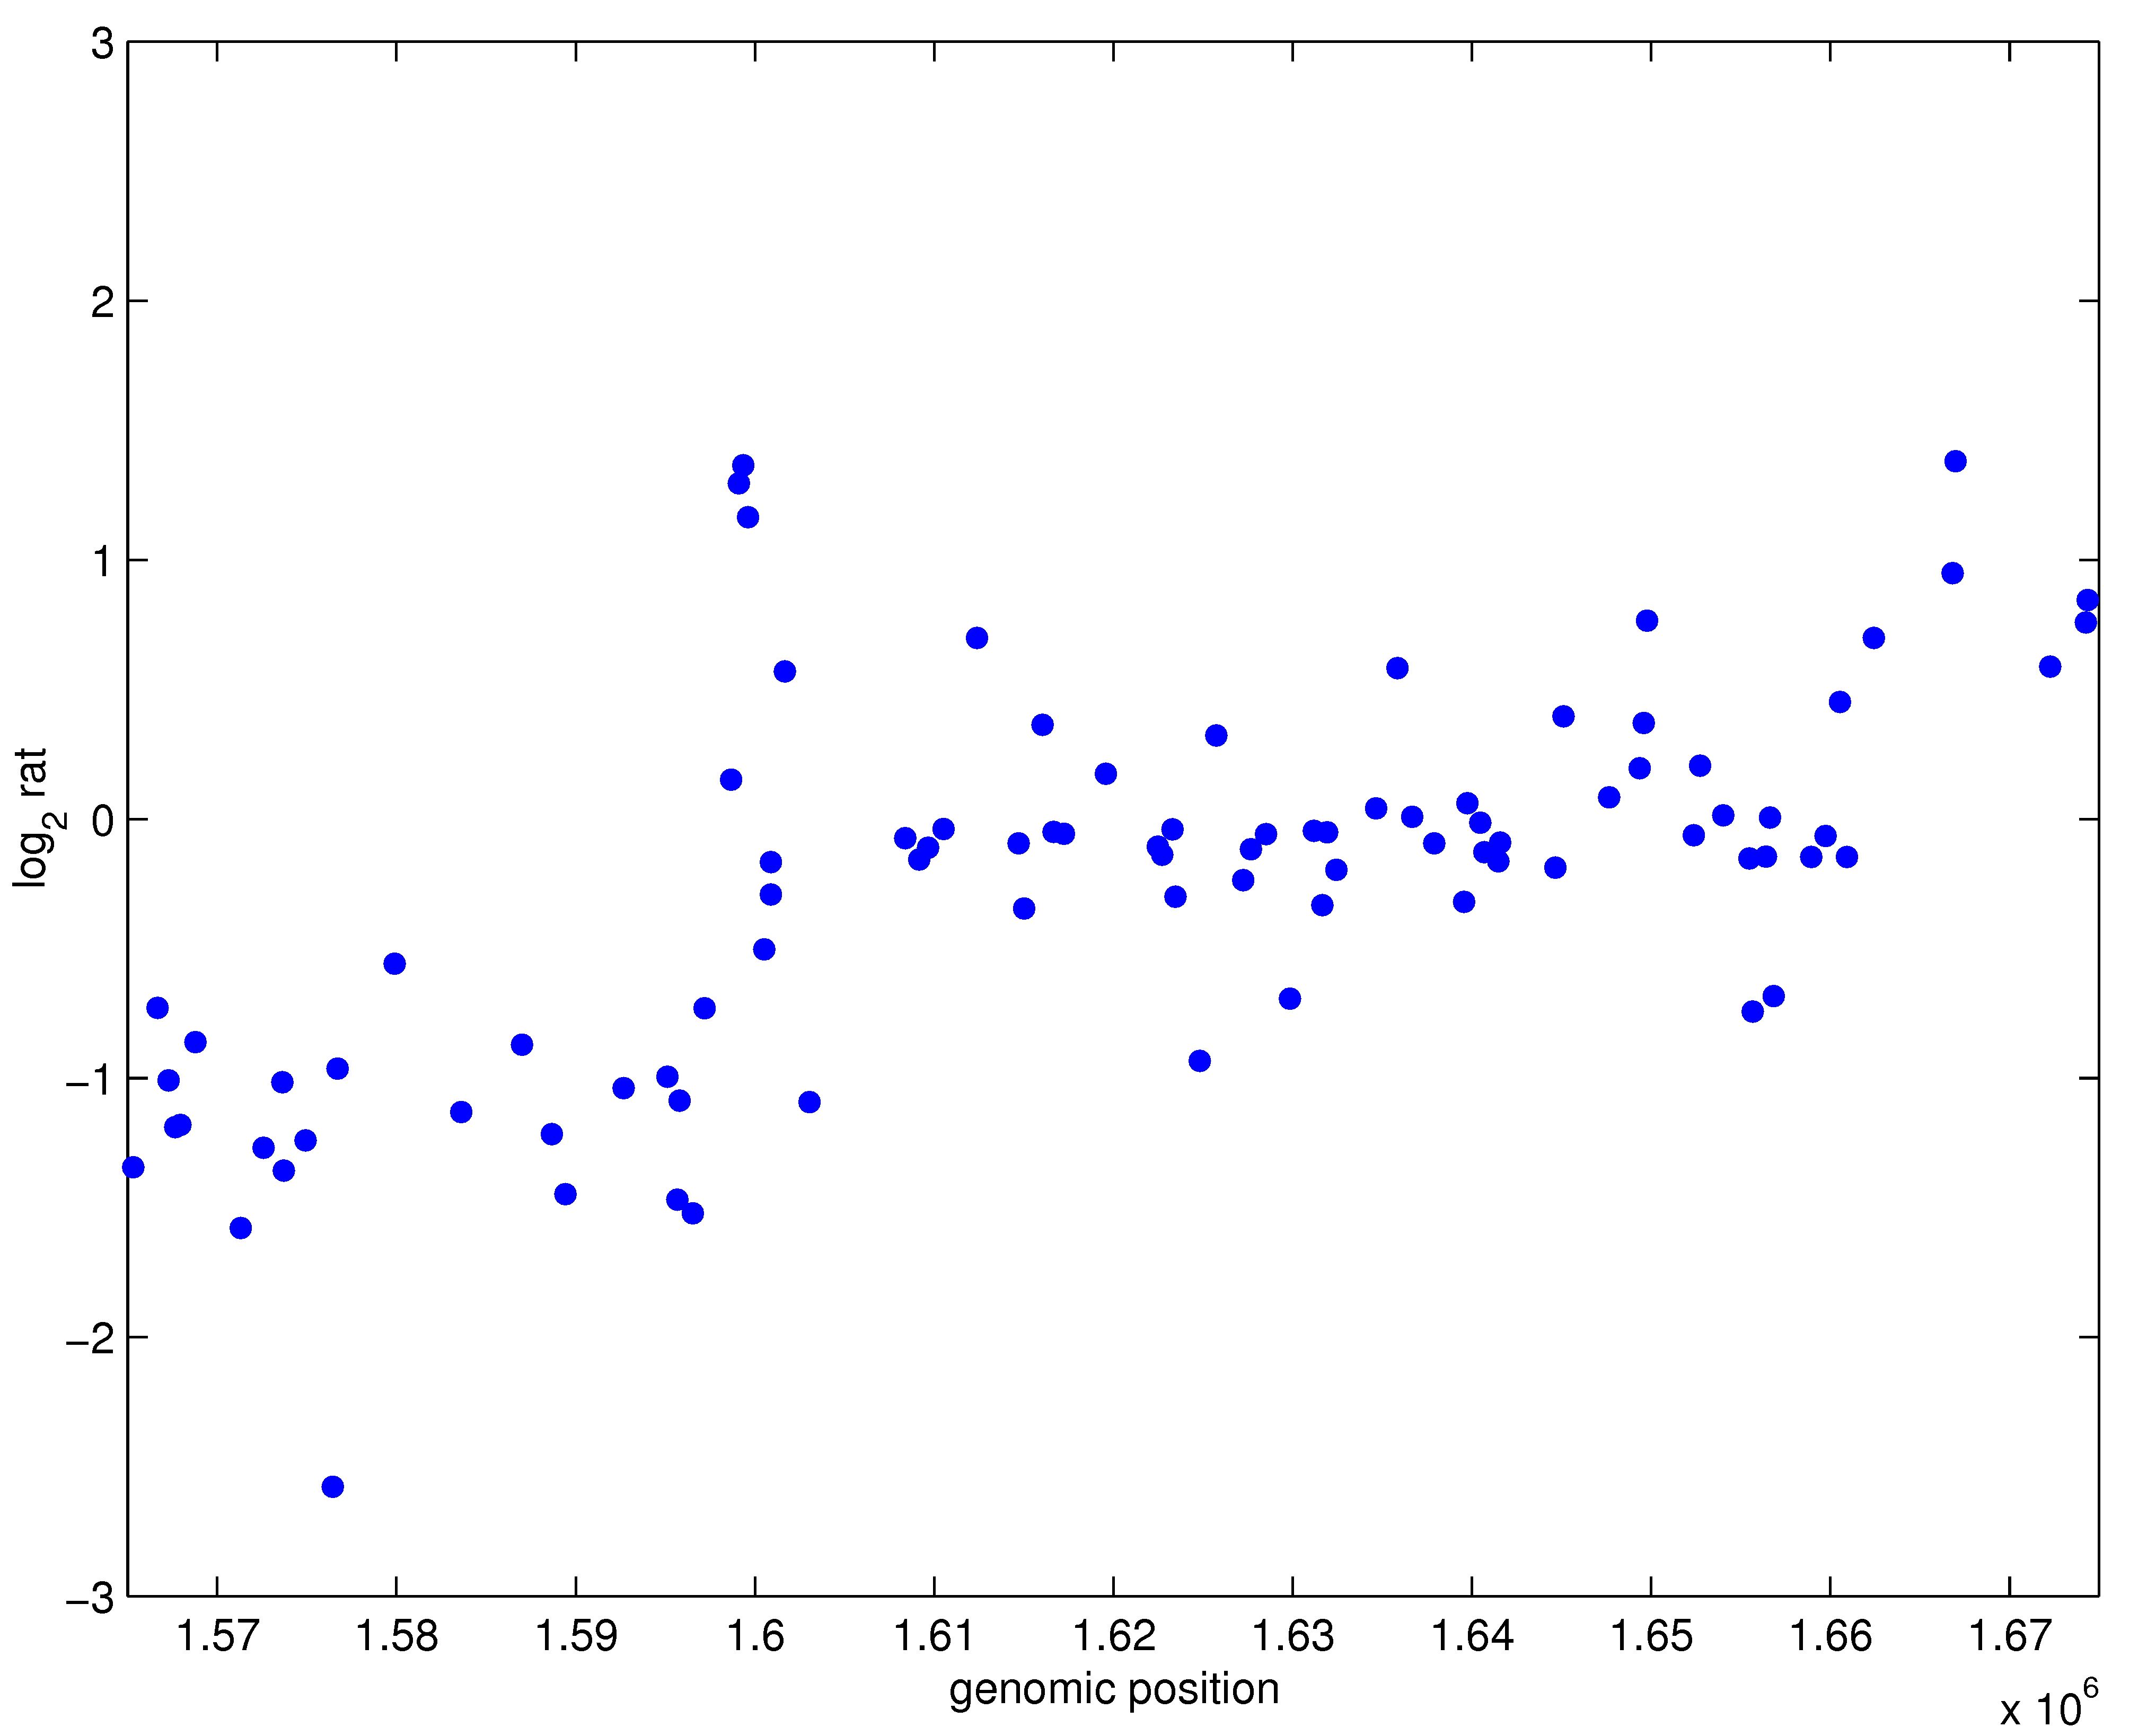
\epsfig{file = ../Figures/raw_profile_example.eps, clip=,
          width=.45\textwidth, height=.5\textheight}  
        \onslide<4>
        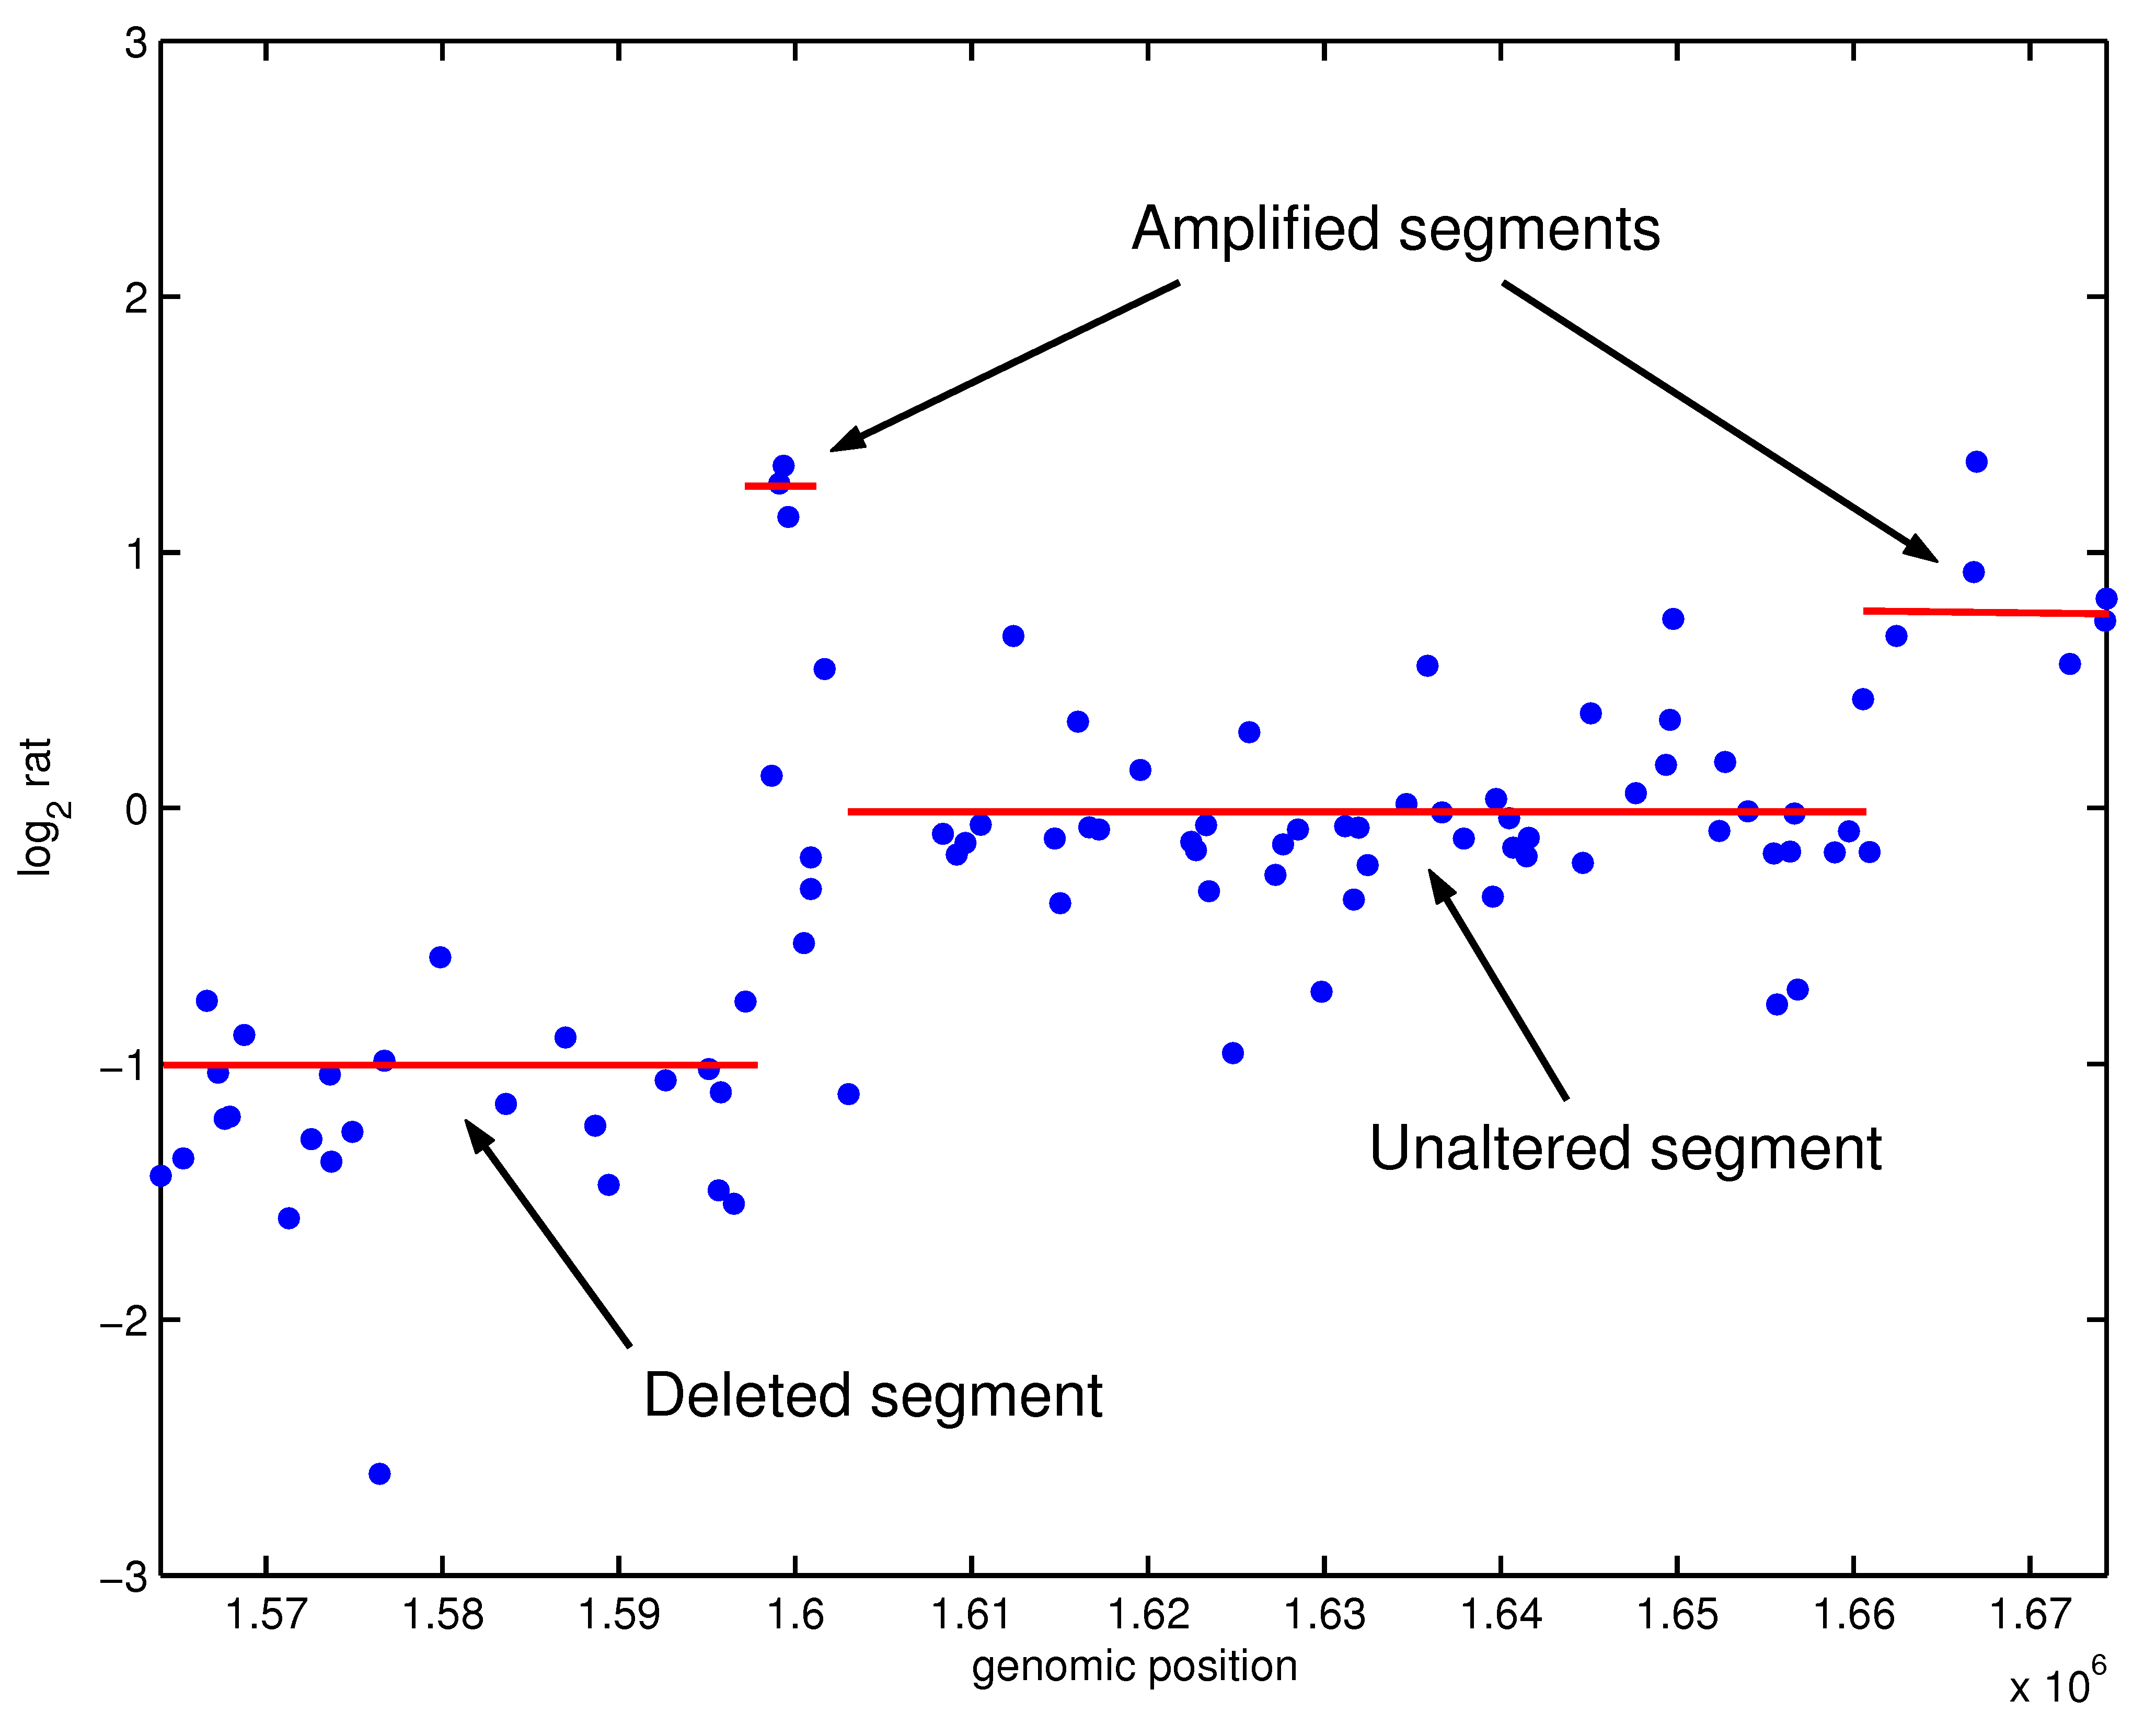
\epsfig{file = ../Figures/profile_example.eps, clip=,
          %bbllx=60, bblly=196, bburx=543, bbury=586}
          width=.45\textwidth, height=.5\textheight}  
      \end{overprint}
    \end{tabular}
  \end{tabular} \\
  \onslide+<3->{
    \begin{eqnarray*}
      Y_t & \propto & f(\text{\emphase{relative copy number} at position }t) \\
      & = & \text{log-fluorescence, sum of the two allele signals for a given
        SNP, etc.}
    \end{eqnarray*}
    }
  }

%====================================================================
%====================================================================
\section{Segmentation model for one profile}
\frame{\frametitle{Segmentation model for one profile}}
%====================================================================

%====================================================================
\subsection*{Statistical model}
%====================================================================
\frame{\frametitle{A model, what for?}
  
  \begin{itemize}
  \item To \emphase{translate biological questions into mathematical
      equations} and quantities;
  \item To make \emphase{all hypotheses explicit};
  \item To set the inference of interesting parameters in a
    \emphase{global framework}, possibly accounting for other effects
    (covariates);
  \item To \emphase{motivate all calculations} and data processing to
    come.
  \end{itemize}
  
  \bigskip\pause
  \centerline{\emphase{The model is the place where biologist's and
      mathematician's minds meet.}}
  
  \bigskip\bigskip\pause
  \paragraph{Model-based approach.}
  \begin{itemize}
  \item Define a model that describes the biological process as well
    as possible;
  \item Make sure that it can be handled in terms of mathematics /
    statistics;
  \item Derive an (efficient and statistically valid) inference
    procedure.
  \end{itemize}
}

%====================================================================
\frame{\frametitle{One Series} \pause
  
  \begin{tabular}{cc}
    \hspace{-.5cm}
    \begin{tabular}{p{.5\textwidth}}
      \onslide+<2->{\paragraph{Statistical model.} 
        \begin{itemize}
        \item $\text{Signal} = f(\text{Position})$; \\}
        \onslide+<3->{
        \item Breakpoint positions: \\
          $\tau_1, \tau_2, ..., \tau_{K-1};$ \\}
        \onslide+<4->{
        \item Mean signal (relative copy number) within each interval: \\
          $\mu_1, \mu_2, ..., \mu_K$; \\}
        \onslide+<5->{
        \item Observed signal (log-ratio) at time $t=$ \\
          mean + i.i.d. noise $\Ncal(0, \sigma^2)$.
        \end{itemize}}
    \end{tabular}
    & 
    \hspace{-1cm}
    \begin{tabular}{c}
      \begin{overprint}
        \onslide<2>
        $\qquad \qquad \;\;\, Y_t =$ \\
        \epsfig{file=../Figures/FigSeg-Budapest-1.eps, clip=,
          angle=270, width=.5\textwidth} 
        \onslide<3>
        if $t \in \textcolor{blue}{I_k}, \quad Y_t =$ \\
        \epsfig{file=../Figures/FigSeg-Budapest-2.eps, clip=,
          angle=270, width=.5\textwidth} 
        \onslide<4>
        if $t \in \textcolor{blue}{I_k}, \quad Y_t = \textcolor{red}{\mu_k}$ \\
        \epsfig{file=../Figures/FigSeg-Budapest-3.eps, clip=,
          angle=270, width=.5\textwidth} 
        \onslide<5->
        if $t \in \textcolor{blue}{I_k}, \quad Y_t =
        \textcolor{red}{\mu_k} + E_t$ \\ 
        \epsfig{file=../Figures/FigSeg-Budapest-4.eps, clip=,
          angle=270, width=.5\textwidth} 
      \end{overprint}
    \end{tabular}
  \end{tabular}
  
  \onslide+<6->{
    \paragraph{Aim:}
    Retrieve the 'true' number of segments \emphase{$K$},
    change-points locations \emphase{$(\tau_k)$} and means
    \emphase{$(\mu_k)$} ... within a reasonable time.
  }
  
}

%====================================================================
\frame{\frametitle{Statistical model} 
  
  \begin{itemize}
  \item Breakpoints = partition of the data into $K$ segments:
    $$
    \tau_1, \tau_2, \dots, \tau_{K-1}
    \qquad \rightarrow \qquad
    I_k=]\tau_{k-1},\tau_k].
    $$
  \item The observed data $\{Y_t\}$ are \emphase{independent}.
  \item The distribution's parameters are \emphase{constant between
      two breakpoints}:
    $$
    \begin{array}{c}
      \text{if position $t$} \\
      \text{is in segments $I_k$:}
    \end{array}
    \quad 
    \left\{ 
      \begin{array}{rcll}
        Y_t & \sim & \Ncal(\mu_k,\sigma^2)  & \text{aCGH (same
          variance)} \\
        \\
        Y_t & \sim & \Ncal(\mu_k,\sigma_k^2)  & \text{aCGH (heter.
          variance)} \\  
        \\
        Y_t & \sim & \Pcal(\mu_k)  &  \text{NGS} \\
        \\
        Y_t & \sim & \Ncal\Bcal(\mu_k, \phi)  &  \text{NGS (over-dispersed)}
      \end{array}
    \right.
    $$
  \end{itemize}
  }

%====================================================================
\frame{\frametitle{Maximum likelihood} 

  To get estimate of the parameters of this model: 
  $$
  T  =  (\tau_1, ..., \tau_{K-1}),
  \qquad
  \Theta  = (\theta_1,\hdots,\theta_K), \quad \theta_k = (\mu_k,
  \sigma_{(k)}^2, \phi, ...)
  $$
  we choose to maximize the likelihood of the observed data:
  $$
  P(\Ybf; T; \Thetabf) = \prod_k \prod_{t \in I_k} p(Y_t, \theta_k)
  $$

  \bigskip\pause
  \paragraph{Array CGH.} Gaussian with same variance $\Ncal(\mu_k, \sigma^2)$:
  $$
  \log P(\Ybf; T; \Thetabf) = \text{cst} - \frac{n}2 \log \sigma^2 -
  \frac1{2 \sigma^2} \sum_k \sum_{t \in I_k} (Y_t - \mu_k)^2
  $$
  
  \bigskip\pause  
  \paragraph{NGS.} Poisson $\Pcal(\mu_k)$:
  $$
  \log P(\Ybf; T; \Thetabf) = \text{cst} - \sum_k \sum_{t \in I_k}
  (\mu_k - Y_t \log \mu_k)
  $$
  }
  
%====================================================================
\subsection*{Parameter inference}

%====================================================================
\frame{\frametitle{Parameter inference} 

  \paragraph{When the breakpoints are known,} estimating the
  parameters is (generally) an easy task. 

  \begin{itemize}
  \item Mean:
    $$
    \widehat{\mu}_k = \frac1{n_k} \sum_{t \in I_k} Y_t
    $$
    where $n_k = \tau_k - \tau_{k-1} = \#$ points in segments $I_k$.
  \item Variance:
    $$
    \begin{array}{lrcl}
      \text{same for all segments:} & \widehat{\sigma}^2 & = &
      \displaystyle{\frac1{n} \sum_{k=1}^K \sum_{t \in I_k} (Y_t -
      \widehat{\mu}_k)^2} \\
    \\
      \text{specific to each segment:} & \widehat{\sigma}^2_k & = &
      \displaystyle{\frac1{n_k} \sum_{t \in I_k} (Y_t - \widehat{\mu}_k)^2}
    \end{array}
    $$
\end{itemize}
}\label{Page:ParamInfer}

%====================================================================
\subsection*{Dynamic programming}
%====================================================================
\frame{\frametitle{Finding the breakpoints} 
  
  When $K$ is known, we aim at minimizing some contrast function
  $$
  J_K(1, n) = \left\{
    \begin{array}{ll}
      \displaystyle{\sum_{k=1}^K \sum_{t \in I_k} (Y_t -
        \widehat{\mu}_k)^2} & \text{for } \Ncal(\mu_k, \sigma^2)\\
      \displaystyle{\sum_{k=1}^K \sum_{t \in I_k} (\widehat{\mu}_k -
        Y_t  \log\widehat{\mu}_k)}  & \text{for } \Pcal(\mu_k)
    \end{array}
  \right.
  $$

  \pause
  \paragraph{Problem.} There are $ \binom{n-1}{K-1} $ possible choices
  for the positions of the breakpoints $\tau_1, \tau_2, \dots,
  \tau_{K-1}$.
  $$
  \text{For } n=1\,000, \qquad K = 20 \quad \longrightarrow \quad
  \binom{n-1}{K-1} \simeq 10^{40}
  $$
  \ra Impossible to explore for large $n$ and $K$
}

%====================================================================
\frame{\frametitle{Shortest path problem}

  \paragraph{Cost of segment.} Define the cost of segment $I= [i, j]$ as
  $$
  C(i, j) = C(I) = \sum_{t \in I} (Y_t - \widehat{\mu}_k)^2 
  \qquad \text{or} \qquad 
  \sum_{t \in I} (\widehat{\mu}_k - Y_t \log\widehat{\mu}_k).   
  $$

  \pause
  \paragraph{Shortest path problem.} The minimization of 
  $$
  J_K(1, n) = \sum_k C(\tau_{k-1}+1, \tau_k)
  $$
  turns out to be a shortest path problem, that is to find the path
  \begin{itemize}
  \item going from 1 to $n$,
  \item in $K$ steps: $[0, \tau_1], [\tau_1+1, \tau_2], ... [\tau_K+1, n]$,
  \item for the smallest possible cost $\widehat{J}_K(1, n)$.
  \end{itemize}
 }

%====================================================================
\frame{\frametitle{Dynamic programming}

  \paragraph{Exact solution.} This shortest path problem can be solve
  thanks to the following dynamic programming algorithm.

  \begin{itemize}
  \item \pause First note that
    $$
    \widehat{J}_1(i, j) = C(i, j);
    $$
  \item \pause Then clearly
    $$
    \widehat{J}_2(1, j) = \min_i C(1, i) + C(i+1, j);
    $$
  \item \pause And finally (Bellman's principle)
    $$
    \widehat{J}_k(1, j) = \min_i \widehat{J}_{k-1}(1, i) + C(i+1, j);
    $$
  \end{itemize}

  \pause
  \paragraph{Complexity.} This algorithm requires
  \begin{itemize}
  \item $O(K n^2)$ computational time and
  \item $O(Kn)$ memory space.
  \end{itemize}
 }

%====================================================================
\frame{\frametitle{Fastening the DP algorithm}

  \paragraph{Quadratic complexity} $O(Kn^2)$ is not acceptable for very
  large signals (e.g. NGS for DNAseq where $n = 10^6$ to $10^8$.

  \pause
  \begin{tabular}{cc}
    \hspace{-.5cm}
    \begin{tabular}{p{.5\textwidth}}
      \begin{itemize}
      \item \emphase{'Pruned DP'} can strongly reduce the
        computational burden (\refer{Rig10}).
      \item Its theoretical worst complexity is the same as regular
        DP.
      \item Its mean empirical complexity is \emphase{almost
        linear: $O(K n \log n)$}.
      \end{itemize} \\
      ~\\
    \end{tabular}
    &
    \hspace{-.5cm}
    \begin{tabular}{p{.5\textwidth}}
    \epsfig{file = ../Figures/Rig10-Fig.ps, clip=, bbllx=290,
      bblly=20, bburx=560, bbury=270, width=.4\textwidth}     
    \end{tabular}
  \end{tabular}

  \pause
  \paragraph{Trick.} Not to compute parameter estimates (see slide
  \ref{Page:ParamInfer}) before to perform segmentation.  \\
  \ra Only applicable for 'nice' contrasts (e.g. Gaussian, Poisson,
  negative binomial with known $\phi$, ...)
}

%====================================================================
\subsection*{Model selection}
%====================================================================
\frame{\frametitle{Model selection: $K = ?$} 

  \paragraph{How many segments?}
  The fit of the segmentation improves as $K$ increases.

  %\bigskip 
  \begin{tabular}{cc}
    \hspace{-.5cm}
    \begin{tabular}{c}
      $\widehat{J}_K(1, n)$ as a function of $K$ \\
      \epsfig{file = ../Figures/Select_K.ps, clip=, bbllx=146, bblly=529,
        bburx=464, bbury=777, height=.35\textwidth, width=.4\textwidth} 
    \end{tabular} \pause
    &
    \hspace{-1cm}
    \begin{tabular}{p{.55\textwidth}} 
      \emphase{Numerous criteria} have been proposed.
      \begin{itemize}
      \item \pause Segmentation is a non standard case \\
        \ra AIC or BIC do not apply;
      \item \pause Penalized contrast \refer{Lav05,Leb05}:
        $$
        \widehat{J}_K(1, n) + \beta \pen(K)
        $$
      \item \pause modified BIC \refer{ZhS07};
      \item \pause ICL \refer{RLR11};
      \end{itemize}
    \end{tabular}
  \end{tabular}

  This turns out to be the \emphase{most delicate problem} in
  practice...   \\
  (see later, on slide \ref{Page:Lasso}).
}

%====================================================================
\frame{\frametitle{What about calling?}

  \paragraph{Calling.} We'd like segments of same type ('normal',
  'loss', gain', {\sl etc.}) to be gathered into groups \ra
  classification problem.

  \bigskip
  \begin{tabular}{cc}
    \hspace{-0.5cm}
    \pause
    \begin{tabular}{p{.5\textwidth}}
      Pure segmentation \\
      \epsfig{file = ../Figures/FigSegClas-1.eps, clip=,
        width=0.45\textwidth, height=0.25\textwidth}
    \end{tabular} 
    &
    \hspace{-1cm}
    \pause
    \begin{tabular}{p{.5\textwidth}}
      Segmentation + classification \\
      \epsfig{file = ../Figures/FigSegClas-2.eps, clip=,
        width=0.45\textwidth, height=0.25\textwidth}
    \end{tabular}
  \end{tabular}

  \bigskip\pause
  \paragraph{Exercise.}
  \begin{itemize}
  \item Write the statistical model allowing to do so 
    (hint: see \refer{PRL07}). 
  \item Or use HMM (see slide  \ref{Page:HMM}).
  \end{itemize}
  }

%====================================================================
\frame{\frametitle{An example: BT474 cell line}

  \paragraph{Chromosome 9.} (An easy case)

  \bigskip
  \begin{tabular}{cc}
    \hspace{-0.5cm}
    \onslide+<1->
    \begin{tabular}{c}
      Homogeneous variances \\
      $\widehat{K}=4$ segments \\ 
      \epsfig{file = ../Figures/bt474_c9_seg_homo_K4.eps, clip=,
        height=.4\textheight, width=.45\textwidth} 
    \end{tabular}
    &
    \hspace{-.5cm}
    \begin{overprint}
      \onslide<2>
      \begin{tabular}{c}
      Heterogeneous variances \\
      $\widehat{K}=4$ segments \\ 
      \epsfig{file = ../Figures/bt474_c9_seg_hetero_K4.eps, clip=, 
        height=.4\textheight, width=.45\textwidth} 
      \end{tabular}
      \onslide<3>
      \begin{tabular}{c}
        Heterogeneous variances + calling \\
        $\widehat{K}=8$ segments \\ 
        \epsfig{file = ../Figures/bt474_c9_segclas_homo_P3K4 , clip=, 
          height=.38\textheight, width=.4\textwidth} 
      \end{tabular}
    \end{overprint}
  \end{tabular}
  }

%====================================================================
\frame{\frametitle{An example: BT474 cell line}

  \paragraph{Chromosome 1.} (An more complex case)

  \bigskip
  \begin{tabular}{cc}
    \hspace{-0.5cm}
    \onslide+<1->
    \begin{tabular}{c}
      Homogeneous variances \\
      $\widehat{K}=10$ segments \\ 
      \epsfig{file = ../Figures/bt474_c1_seg_homo_K10.eps, clip=, 
        height=.4\textheight, width=.45\textwidth} 
    \end{tabular}
    &
    \hspace{-.5cm}
    \begin{overprint}
      \onslide<2>
      \begin{tabular}{c}
        Heterogeneous variances \\
        $\widehat{K}=2$ segments \\ 
        \epsfig{file = ../Figures/bt474_c1_seg_hetero_K2.eps, clip=,
          height=.4\textheight, width=.45\textwidth} 
      \end{tabular}
      \onslide<3>
      \begin{tabular}{c}
        Heterogeneous variances + calling \\
        $\widehat{K}=8$ segments \\ 
        \epsfig{file = ../Figures/resultat_P3K8.eps , clip=, 
          height=.38\textheight, width=.43\textwidth} 
      \end{tabular}
    \end{overprint}
  \end{tabular}
  }

%====================================================================
%====================================================================
\section{Segmentation of multiple profiles}
\frame{\frametitle{Segmentation of multiple profiles}}
%====================================================================
\frame{\frametitle{Multiple profiles}
  
  \begin{tabular}{cc}
    \begin{tabular}{p{6cm}}
      Cancer studies often involve CGH profiles of numerous
      patients ($m \approx 100$). \\
      \bigskip
      Even when having the same disease, patients generally
      \emphase{do not have common breakpoints}.\\
      \bigskip
      Simultaneous analysis of all profiles $\{Y_{it}\}$ allows
      to \emphase{correct for artifacts} such as probe effect.\\
        \bigskip
      \refer{PLB11}
    \end{tabular}    
    &
    \begin{tabular}{p{6cm}}
      \hspace{-.75cm}
      \epsfig{file = ../Figures/nakao-mat.txt-MixSeg-V2.eps, bbllx=90,
      bblly=220, bburx=380, bbury=590, clip=, scale=.5}
    \end{tabular}
  \end{tabular}
  }

%====================================================================
\subsection*{Statistical model}
%====================================================================
\frame{\frametitle{Statistical model}

  \paragraph{Notation.}
  \begin{itemize}
  \item $Y_{it} = $ signal for patient $i$ ($i = 1..m$) at position
    $t$ ($t = 1..n$);
  \item $K_i = $ number of segments of patient $i$;
  \item $I_{ik} = k$-th segment of patient $i$ ($k = 1.. K_i$).
  \end{itemize}

  \bigskip\pause
  \paragraph{Model.} Data are independent, 
  $$
  \text{if }t \in I_{ik}, \qquad Y_{it} \sim \Ncal(\mu_{ik} + \beta_t,
  \sigma^2)
  $$
  where $\beta_t$ stands for the \emphase{probe effect} at position
  $t$.  

  \bigskip\pause
  \paragraph{Remark.} The model can be written as a \emphase{linear
    model}:
  $$
  \Ybf = \Tbf  \mubf + \Xbf \betabf + \Ebf
  $$
  ... where the segmentation matrix $\Tbf$ is unknown.
}\label{Page:MultiModel}

%====================================================================
\subsection*{Inference}
%================================================\pause====================
\frame{\frametitle{Statistical inference}

  \paragraph{Segmentation.} DP can be generalized (2-stage DP
  algorithm) to perform the segmentation of multiple profiles with a
  fixed total number of segments $K_+ = \sum_i K_i$.

  \bigskip\bigskip\pause
  \paragraph{Model selection.} Criteria used for one single profile
  can be generalized as well.

  \bigskip\bigskip\pause
  \paragraph{Parameter estimation.} The mean of each segments
  ($\mu_{ik}$) and the probe effect ($\beta_t$) must can be estimated
  in an iterative way:
  \begin{eqnarray*}
    \emphase{\mu^{h+1}_{ik}}  & = & \arg\min_{\mu_{ik}} \sum_i \sum_k \sum_{t \in
      I_{ik}} (Y_{it} - \mu_{ik} - \emphase{\beta^h_t})^2, \\
    \emphase{\beta_t^{h+1}} & = & \arg\min_{\beta_t} \sum_i \sum_k \sum_{t \in
      I_{ik}} (Y_{it} - \emphase{\mu^{h+1}_{ik}} - \beta_t)^2. \\
  \end{eqnarray*}

}

%====================================================================
\subsection*{CGHseg R-package}
%====================================================================
\frame{\frametitle{CGHseg R-Package} 

  \paragraph{CGHseg} is an R package dedicated to the analysis of
  Comparative Genomic Hybridization (\refer{PLH11}). 
  
  \bigskip\pause
  \paragraph{Linear model framework:} 
 
  \medskip
  \begin{tabular}{p{.2\textwidth}p{.35\textwidth}p{.35\textwidth}}
%     \emphase{Task} & \emphase{Representation} & \emphase{Model} \\   
%     \hline
%     \\
    \emphase{Segmentation} & regression on unknown $\Tbf$: &
    $\displaystyle{\Ybf = \Tbf \mubf + \Ebf}$ \pause \\ 
    \\
    \emphase{Correction} & fixed covariates effect: $\betabf$ &
    $\displaystyle{\Ybf = \Tbf \mubf + \Xbf \betabf + \Ebf}$ \pause \\  
    \\
    \emphase{\sl Correlation}\footnote{\refer{PLB11}} & {\sl random
      probe effect: $\Ubf$}  & 
    $\displaystyle{\sl \Ybf = \Tbf \mubf + \Zbf \Ubf + \Ebf}$  \pause \\ 
    \\
    \emphase{Calling} & cross-tabulation table $\Cbf$: &
    $\displaystyle{\Ybf = \Tbf \Cbf \mbf + \Ebf}$ \pause \\
    \\
    \emphase{Combinations} 
    & fixed + random effects: &
    $\displaystyle{\Ybf = \Tbf \mubf + \Xbf \betabf + \Zbf \Ubf + \Ebf}$ \\
    & fixed effects + calling: &
    $\displaystyle{\Ybf = \Tbf \Cbf \mbf + \Xbf \betabf + \Ebf}$  \\
  \end{tabular}
}


%====================================================================
\frame{\frametitle{An example of combination}

  \begin{tabular}{ccc}
    \onslide+<1->{\textcolor{red}{Segmentation}
      % +\textcolor{green}{calling}
    }
    & 
    \onslide+<2->{+ \textcolor{blue}{fixed effects} }
    & 
    \onslide+<3->{$\Ybf = \textcolor{red}{\Tbf} 
      %\textcolor{green}{\Cbf} 
      \mbf + \textcolor{blue}{\Xbf} \betabf + \Ebf$  }
    \\
    % \epsfig{file = ../Figures/PLH11-V1-Fig1.eps, clip=, angle=270,
    %   bbllx=10, bblly=0, bburx=300, bbury=840, scale=0.4}        
    \onslide+<1->{\epsfig{file = ../Figures/PLH11-V1-Fig1.eps, clip=,
        angle=270, bbllx=33, bblly=34, bburx=282, bbury=272,
        scale=0.4}}   
    & 
    \onslide+<2->{\epsfig{file = ../Figures/PLH11-V1-Fig1.eps,
        clip=, angle=270, bbllx=33, bblly=302, bburx=282, bbury=540,
        scale=0.4}} 
    & 
    \onslide+<3->{\epsfig{file = ../Figures/PLH11-V1-Fig1.eps, clip=,
        angle=270, bbllx=33, bblly=571, bburx=282, bbury=810,
        scale=0.4}}         
  \end{tabular}

  \bigskip
  \onslide+<4->{
    \begin{itemize}
    \item \emphase{Correction:} functional versions (spline, wavelets)
      for the probe effect.
    \item Several model selection criteria; Default = modified BIC.
%    \item \emphase{Presentation} at
%      \url{www.agrocampus-ouest.fr/math/useR-2009/}
    \item \emphase{\tt cran.r-project.org/web/packages/cghseg/index.html}
    \end{itemize}
  }
  
}

%====================================================================
\frame{\frametitle{Some simulations}

  \vspace{-0.5cm}
  \begin{tabular}{cc}
    \hspace{-0.5cm}
    \begin{tabular}{p{.5\textwidth}}
      Correction and calling improve
      \begin{itemize}
      \item the estimation of $K$, 
      \item the breakpoint detection (FDR / FNR), 
      \item the  recovery of the true signal.
      \end{itemize}
      
      \bigskip
      \paragraph{Calling:} yes = --, no = - -

      \bigskip
      \paragraph{Correction:} \\
      $\blacksquare =$ no correction, \\
      \textcolor{red}{$\bullet = $ position  specific}, \\
      \textcolor{blue}{$\triangle =$ spline}, \\
      \textcolor{green}{$\diamond =$ wavelet}, \\
      \textcolor{orange}{$\circ =$ CBS} 
    \end{tabular}
    &
    \hspace{-1cm}
    \begin{tabular}{p{.5\textwidth}}
      \epsfig{file = ../Figures/PLH11-V1-Fig2.eps, clip=,
        width=.5\textwidth, height=0.85\textheight}        
    \end{tabular}
  \end{tabular}

  }

%====================================================================
%====================================================================
\section{Lasso techniques}
\frame{\frametitle{Lasso techniques}}
%====================================================================

%====================================================================
\subsection*{Convex optimization}
%====================================================================
\frame{\frametitle{An optimization perspective} 

  \vspace{-0.5cm}
  \begin{tabular}{cc}
    \hspace{-0.5cm}
    \begin{tabular}{p{.6\textwidth}}
      \paragraph{Segmentation problem} can be rephrased as
      $$
      \widehat{\mubf}_{\text{Seg}} = \min_{\mubf} \sum_t (Y_t - \mu_t)^2 
      + \lambda \sum_t |\mu_t - \mu_{t-1}|_0 
      $$
      where $|\cdot|_0$ stands for the so-called $\ell_0$ norm:
    \end{tabular}
    &
    \hspace{-1cm}
    \begin{tabular}{p{.35\textwidth}}
      \epsfig{file=../Figures/FigSeg-Budapest-4.eps, clip=,
        angle=270, width=.4\textwidth}       
    \end{tabular}
  \end{tabular}
  \vspace{-.5cm}
  $$
  \sum_t |\mu_t - \mu_{t-1}|_0 = \text{\emphase{number of changes} in
    $\mu_t$} = K-1
  $$
  and $\lambda$ controls the number of segments $K$.
  
  \pause\bigskip
  \paragraph{Remarks.}
  \begin{itemize}
  \item This optimization problem turns out to be
    \emphase{non convex}. 
  \item This prevents the use the huge set of \emphase{convex
      optimization} techniques.
  \item Hopefully, dynamic programming does exist.
  \end{itemize}
}\label{Page:Lasso}

%====================================================================
\frame{\frametitle{Lasso}

  \paragraph{Lasso trick.} Replacing the $\ell_0$ with the
  $\ell_1$ norm makes the optimization problem convex:
  $$
  \widehat{\mubf}_{\text{Lasso}} = \min_{\mubf} \sum_t (Y_t - \mu_t)^2 
  + \lambda \sum_t |\mu_t|
  $$
  that can be solved in \emphase{linear time}.

  \bigskip
  %\vspace{-0.5cm}
  \begin{tabular}{cc}
    \hspace{-0.5cm}
    \begin{tabular}{p{.5\textwidth}}
      \onslide+<2->{
        \paragraph{Regularization:} \\
      }
      \begin{itemize}
        \onslide+<3->{
        \item Due to the $\ell_1$ topology, most of the parameters
          $\mu_t$ are \emphase{set to 0}. \\ ~
        } 
        \onslide+<4->{
        \item The coefficient $\lambda$ controls the \emphase{number of
          non-zero terms}. \\ ~
          }
      \end{itemize}
      \vspace{2cm}
      ~
    \end{tabular}
    &
    \hspace{-.5cm}
    \begin{tabular}{p{.5\textwidth}}
      \begin{overprint}
        \onslide<2>
        \epsfig{file=../Figures/Reg-Lasso0-mu.eps, clip=,
          width=0.6\textwidth}
        \onslide<3>
        \epsfig{file=../Figures/Reg-Lasso1-mu.eps, clip=,
          width=0.6\textwidth}
        \onslide<4->
        \epsfig{file=../Figures/Reg-Lasso2-mu.eps, clip=,
          width=0.6\textwidth}
      \end{overprint}
    \end{tabular}
  \end{tabular}
}

%====================================================================
\frame{\frametitle{Fused Lasso}

  \paragraph{Fused Lasso.} For a segmentation purpose, a second term
  penalizing \emphase{changes among the $\mu_t$} can be added
  (\refer{TSR05}):
  $$
  \widehat{\mubf} = \min_{\mubf} \sum_t (Y_t - \mu_t)^2 
  + \lambda_1 \sum_t |\mu_t| 
  + \lambda_2 \sum_t |\mu_t - \mu_{t-1}| 
  $$
  $$
  \text{where } \sum_t |\mu_t - \mu_{t-1}|_1 = \text{\emphase{sum of
      the absolute changes} in $\mu_t$.}
  $$
  
  \bigskip\pause
  \paragraph{Interpretation.}
  \begin{itemize}
  \item $\sum_t (Y_t - \mu_t)^2$: fit to the observations;
  \item $\lambda_1 \sum_t |\mu_t|$: controls the number of 'abnormal' positions;
  \item $\lambda_2 \sum_t |\mu_t - \mu_{t-1}|$: controls the number of
    breakpoints.
  \end{itemize}
}
 
%====================================================================
\frame{\frametitle{Application to CGH}

  \paragraph{Effect of $w = 2 \lambda_1 / \lambda_2$.}  \refer{TiW08}
  \\ ~\\
  
  \begin{tabular}{c}
    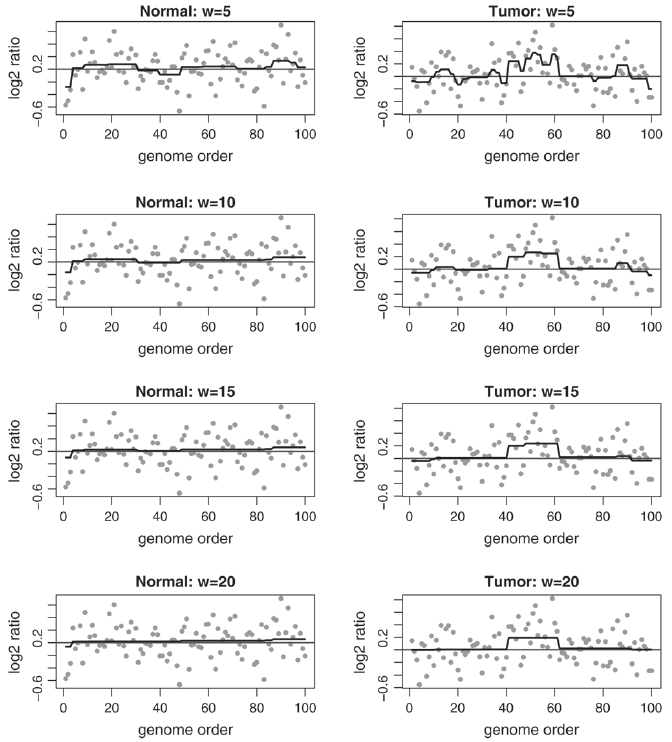
\epsfig{file=../Figures/TiW07-BioStat-Fig2.ps, clip=,
      bblllx=0, bblly=630, bburx=690, bbury=756, 
      width=0.9\textwidth} \\ \pause
    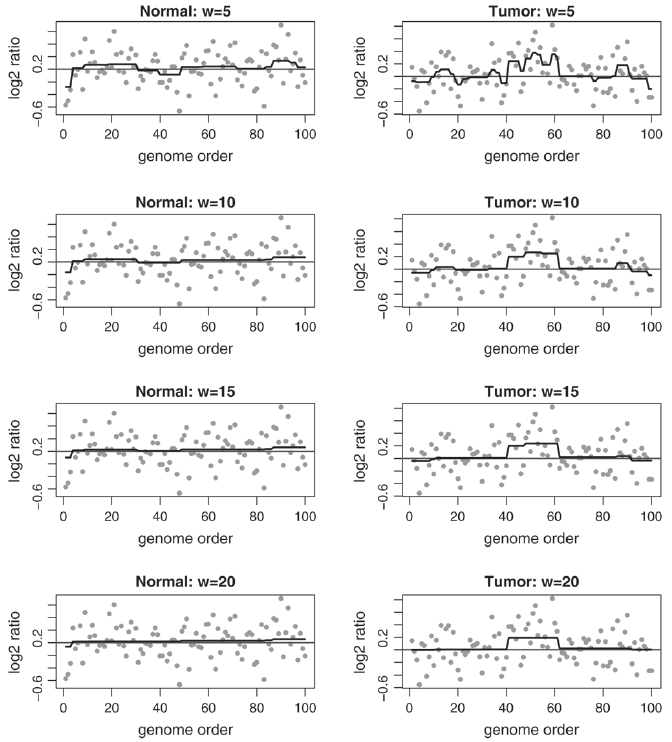
\epsfig{file=../Figures/TiW07-BioStat-Fig2.ps, clip=,
      bblllx=0, bblly=440, bburx=690, bbury=560, 
      width=0.9\textwidth} \\ \pause
    % 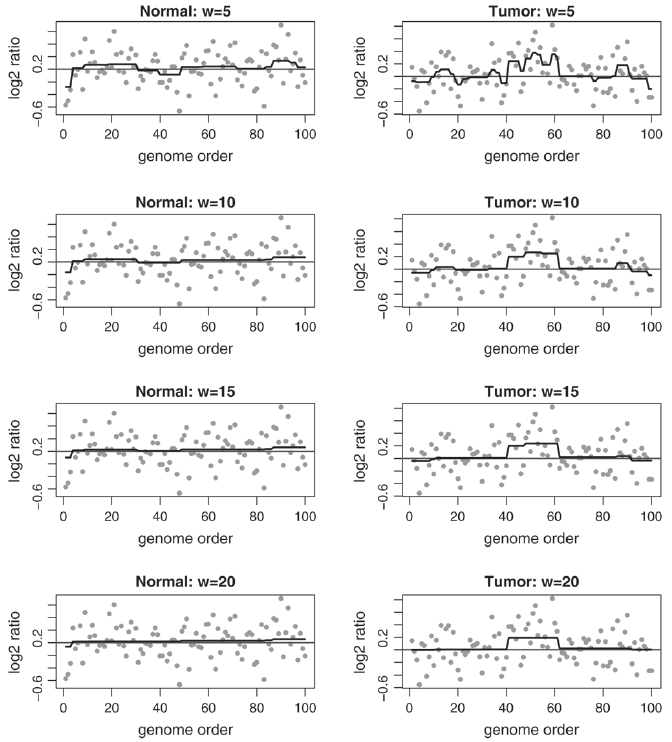
\epsfig{file=../Figures/TiW07-BioStat-Fig2.ps, clip=,
    %   bblllx=0, bblly=250, bburx=690, bbury=370, 
    %   width=0.9\textwidth} \\ \pause
    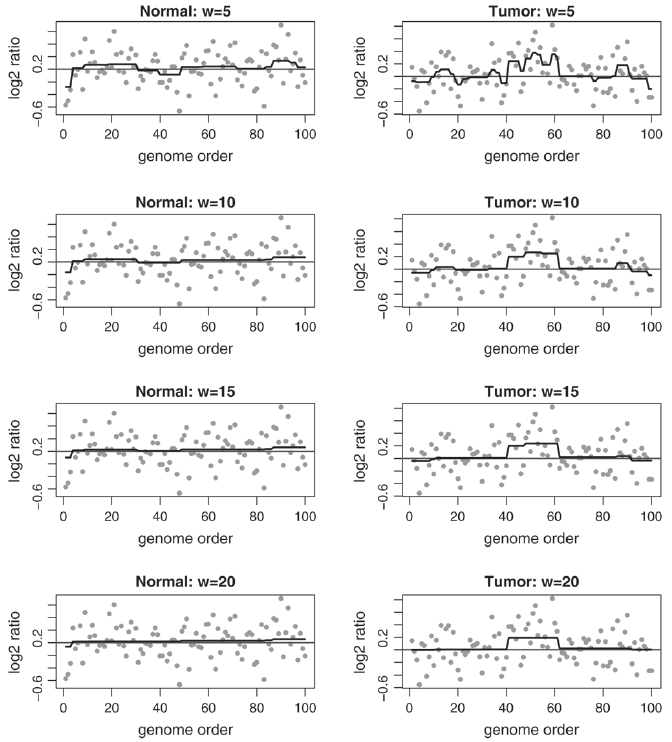
\epsfig{file=../Figures/TiW07-BioStat-Fig2.ps, clip=,
      bblllx=0, bblly=55, bburx=690, bbury=180, 
      width=0.9\textwidth} \\
  \end{tabular}
  }

%====================================================================
\frame{\frametitle{Multiple profiles}

  \paragraph{Aim.} Consider the profiles of $m$ patients (see slide
  \ref{Page:MultiModel}). We'd like to perform segmentation
  \begin{itemize}
  \item for \textcolor{darkgreen}{all patients at the same time},
  \item with a \textcolor{red}{limited number of breakpoints}, 
  \item assuming that they \textcolor{blue}{share similar changes},
  \item within a reasonable time.
  \end{itemize}

  \pause
  %\vspace{-0.5cm}
  \begin{tabular}{cc}
    \hspace{-0.5cm}
    \begin{tabular}{p{.4\textwidth}}
      \paragraph{Playing with penalties.} $\ell_1$ and $\ell_2$ penalties
      can be combined:
      $$
      \min \textcolor{darkgreen}{\sum_i \sum_t (Y_{it} - \mu_{it})^2} 
      $$
      $$
      +
      \lambda \textcolor{red}{\sum_t \textcolor{blue}{\sqrt{\sum_i
            \left(\mu_{i,t} - \mu_{i, t-1}\right)^2}}}
      $$
      \refer{VeB10}
    \end{tabular}
    &
    \hspace{-.5cm}
    \pause
    \begin{tabular}{p{.5\textwidth}}
      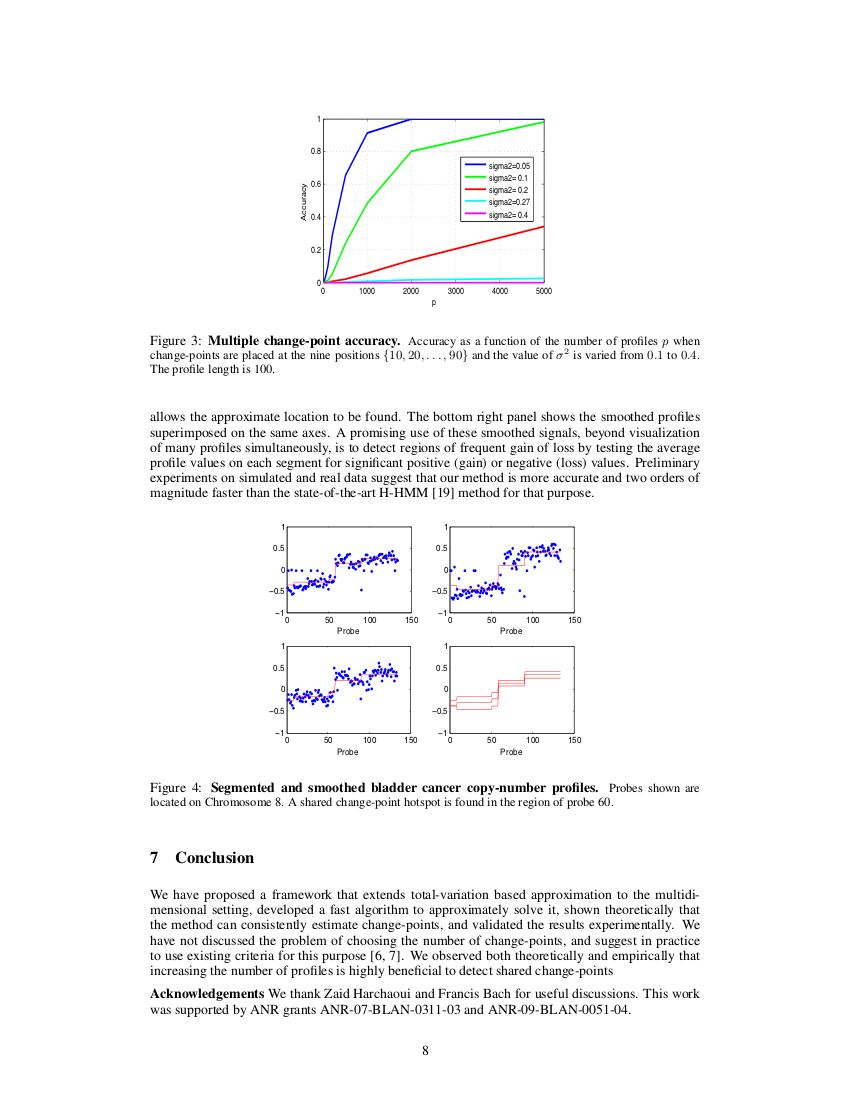
\epsfig{file=../Figures/VeB10-NIPS-Fig4.eps,
        %bblllx=208, bblly=262, bburx=430, bbury=430, 
        width=0.55\textwidth, height=0.55\textheight, clip=}       
    \end{tabular}
  \end{tabular} 
}

%====================================================================
\section{Hidden Markov model}
\frame{\frametitle{Hidden Markov model}}
\label{Page:HMM}
%====================================================================

%====================================================================
\frame{\frametitle{Another model for the same problem}

  \vspace{-0.5cm}
  \begin{tabular}{cc}
    \hspace{-1cm}
    \begin{tabular}{p{.5\textwidth}}
      \begin{itemize}
      \item \onslide+<1->{$t = 1..n$ probes (positions) are observed.}
      \item \onslide+<2->{An \emphase{unobserved label $Z_t$}
          ('loss', '\textcolor{red}{normal}',
          '\textcolor{darkgreen}{gain}') is associated with each probe;}
      \item \onslide+<3->{The distribution of the \emphase{observed signal
          $Y_t$} depends on the label.}
      \item \onslide+<4->{We only observe the signal;}
      \item \onslide+<5->{And we would like to retrieve the 'truth'.}
      \end{itemize}
    \end{tabular}
    &    \hspace{-1cm}
    \begin{tabular}{p{.5\textwidth}}
      \begin{overprint}
        \onslide<1> 
        \epsfig{file=\figSimHMM/SimHMM_n100_Q3.eps,
          width=0.4\textwidth, height=0.7\textheight, angle=270, clip=}
        \onslide<2> 
        \epsfig{file=\figSimHMM/SimHMM_n100_Q3_Z.eps,
          width=0.4\textwidth, height=0.7\textheight, angle=270, clip=}
        \onslide<3> 
        \epsfig{file=\figSimHMM/SimHMM_n100_Q3_ZX.eps,
          width=0.4\textwidth, height=0.7\textheight, angle=270, clip=}
        \onslide<4> 
        \epsfig{file=\figSimHMM/SimHMM_n100_Q3_X.eps,
          width=0.4\textwidth, height=0.7\textheight, angle=270, clip=}
        \onslide<5> 
        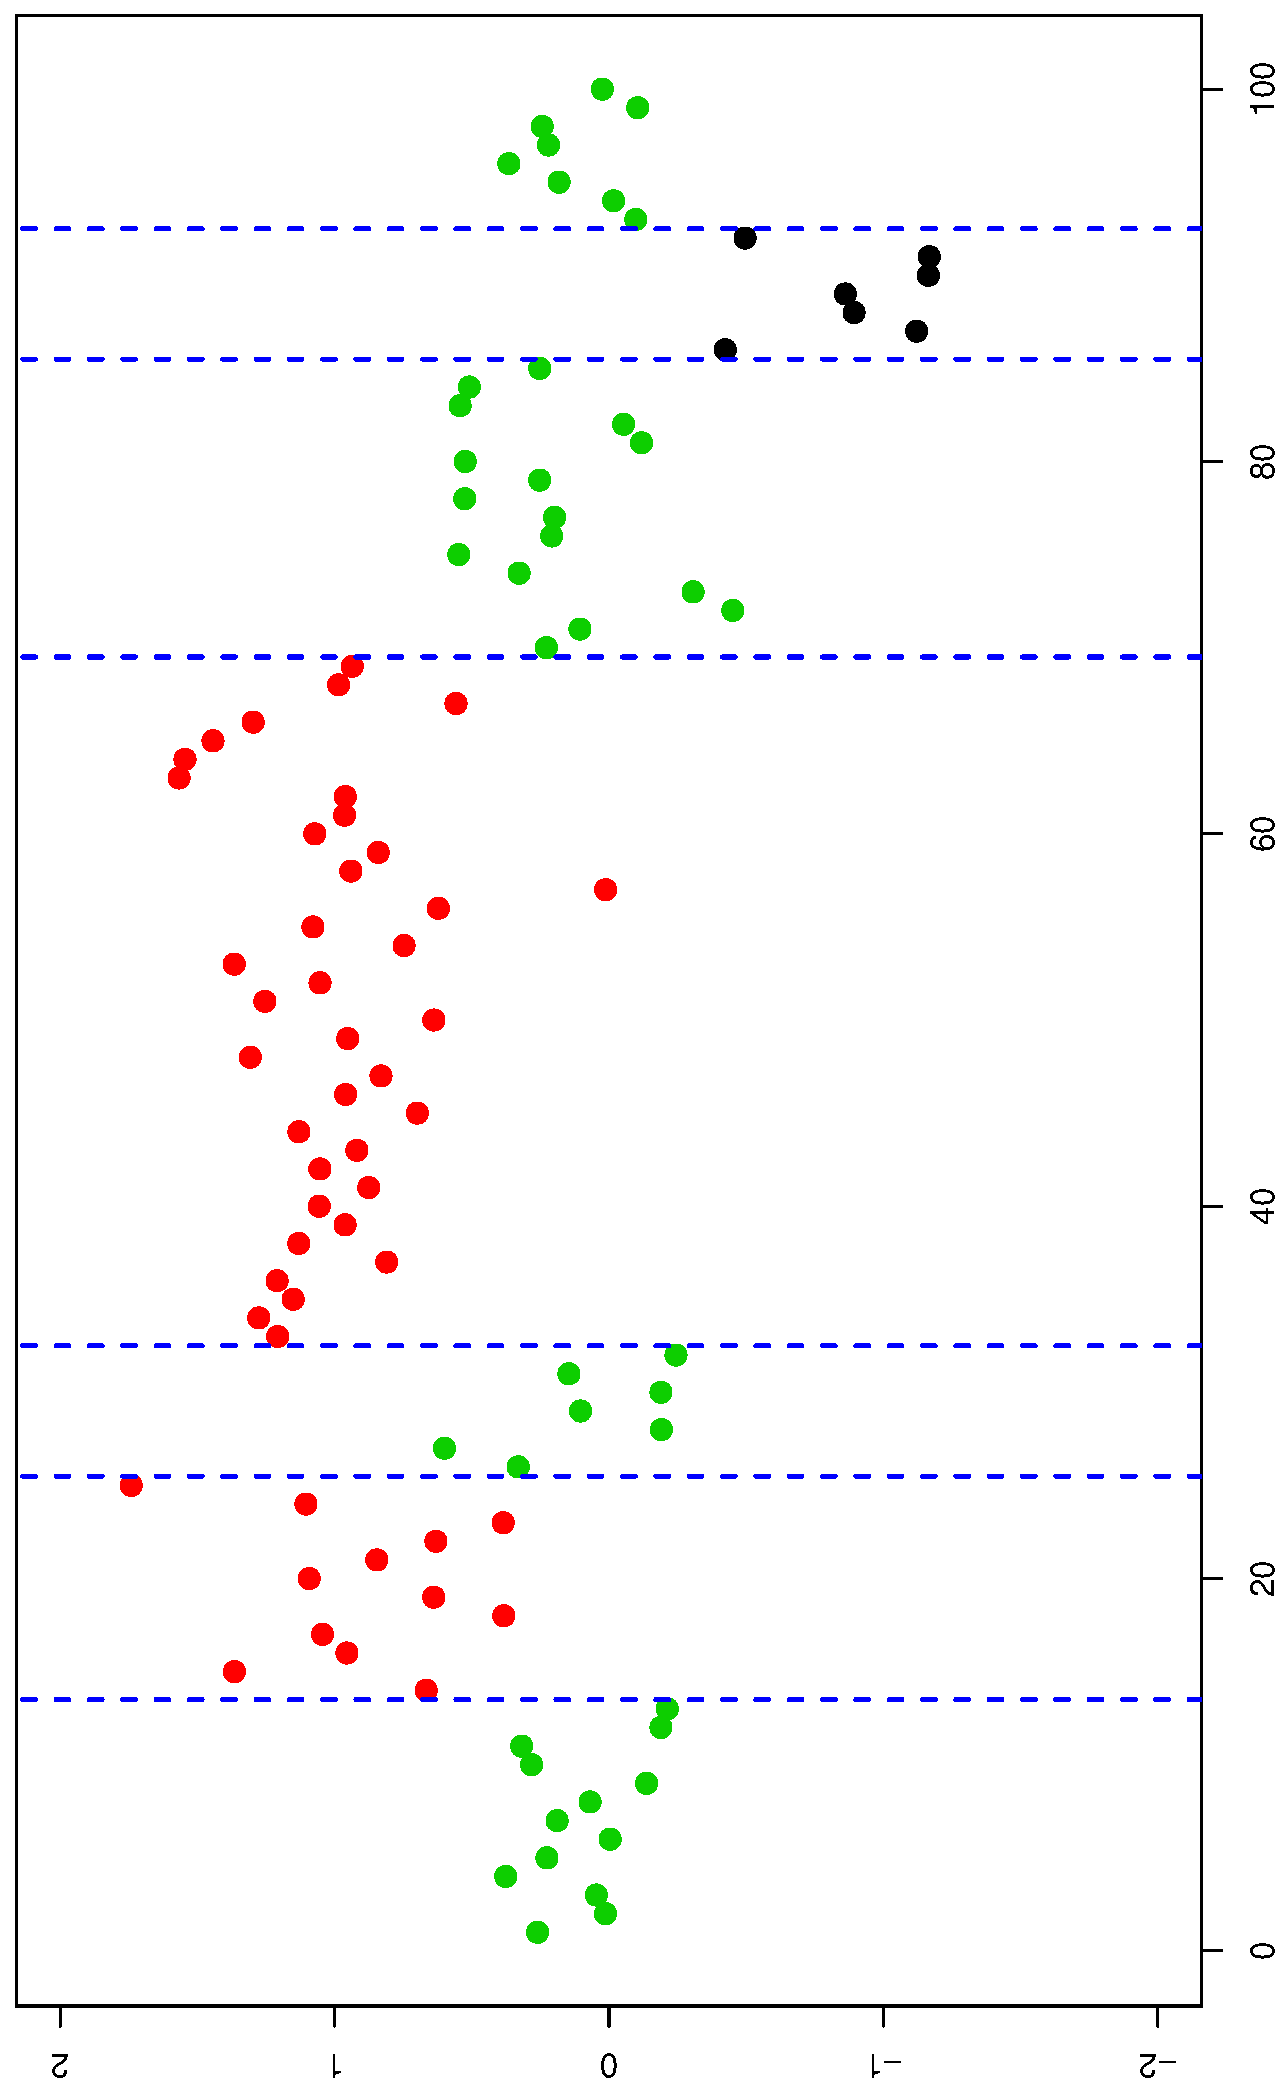
\epsfig{file=\figSimHMM/SimHMM_n100_Q3_ZvitXT.eps,
          width=0.4\textwidth, height=0.7\textheight, angle=270, clip=}
        \onslide<6> 
        \epsfig{file=\figSimHMM/SimHMM_n100_Q3_ZXT.eps,
          width=0.4\textwidth, height=0.7\textheight, angle=270, clip=}
      \end{overprint}
    \end{tabular}
  \end{tabular} \\
  \onslide+<6->{(Although we know we won't succeed.)}
  
}

%====================================================================
\frame{\frametitle{Statistical model}

  \onslide+<1->{
    \paragraph{Hidden labels.} $(Z_t)$ is a Markov chain:
    \begin{itemize}
    \item $Z_t \in \emphase{\{1..Q\}}$, e.g. $Q = 3$ for
      $\{$'loss', 'normal', 'gain'$\}$;
    \item The label of a probe \emphase{depends on the label of the
        preceding} probe:
      $$
      \text{transition probability} \quad \pi_{q\ell} = 
      \Pr\{Z_t = \ell | Z_{t-1} = q\}
      $$
    \end{itemize}
    }
    
    \onslide+<2->{
      \bigskip
      \paragraph{Observed signal.} $(Y_t)$ are independent, given the
      labels $(Z_t)$:
      $$
      \text{if } Z_t = q: \qquad
      Y_t \sim \Ncal(\mu_q, \sigma^2_{(q)})
      \qquad \text{or} \qquad
      Y_t \sim \Pcal(\mu_q).
      $$
    }
    
    \paragraph{Graphical model representation.}
    \begin{overprint}
      \onslide<1>
      $$
      \epsfig{file=../Figures/GM-HMM-ZY.eps,
        bbllx=0, bblly=465, bburx=660, bbury=540,
        width=0.7\textwidth, clip=}
      $$
      \onslide<2>
      $$
      \epsfig{file=../Figures/GM-HMM-ZY.eps,
        bbllx=0, bblly=335, bburx=660, bbury=540,
        width=0.7\textwidth, clip=}
      $$
    \end{overprint}
  }

%====================================================================
\frame{\frametitle{Parameter inference}

  \paragraph{Incomplete data model.} Parameter inference would be easy
  if the labels where known.

  \bigskip\pause
  \paragraph{E-M algorithm.} The most common strategy consist in
  retrieving the missing information.
  \begin{itemize}
  \item \emphase{E-step:} Compute the probability for each probe $t$
    to have label $q$:
    $$
    \tau_{tq} = \Pr\{Z_t = q \;|\; \Ybf\};
    $$
  \item \pause \emphase{M-step:} Estimate the parameters based the
    inferred labels, e.g.
    $$
    \widehat{\mu}_q = \sum_t \tau_{tq} Y_t \left/ \sum_t \tau_{tq} \right..
    $$
  \end{itemize}
  \refer{DLR77}, \refer{CMR05}, \refer{DEK99}
  }

%====================================================================
\frame{\frametitle{Calling}

  \onslide+<1->{
    \paragraph{Probe classification.} Segmentation is finally obtained
    by assigning a label to each probe.
  }
  
  \bigskip
  \begin{tabular}{cc}
    \hspace{-0.5cm}
    \begin{tabular}{p{.5\textwidth}}
      \onslide+<2->{
        \paragraph{MAP rule.} 
        The $\tau_{tq}$ can provide \emphase{maximum a posteriori}
        classification:
        $$
        \widehat{Z}_t = \arg\max_q \tau_{tq}.
        $$ \\
      }
      \onslide+<3->{
        \paragraph{Most probable hidden path.} The succession of the
        MAP $(\widehat{Z}_t)$ is \emphase{not} the most probable
        hidden path:
        $$
        \widehat{\Zbf} = \arg\max_{\Zbf} P(\Zbf|\Ybf) \neq
        (\widehat{Z}_t) 
        $$
        % \begin{eqnarray*}
        %   \widehat{\Zbf} & = & \arg\max_{\Zbf} P(\Zbf|\Ybf) \\
        %   & \neq & (\widehat{Z}_t) 
        % \end{eqnarray*}
      }
    \end{tabular}
    &
    \hspace{-1cm}
    \begin{tabular}{p{.5\textwidth}}
      \begin{overprint}
        \onslide<1> 
        \epsfig{file=\figSimHMM/SimHMM_n100_Q3_X.eps,
          width=0.4\textwidth, height=0.7\textheight, angle=270, clip=}
        \onslide<2> 
        \epsfig{file=\figSimHMM/SimHMM_n100_Q3_ZmapXT.eps,
          width=0.4\textwidth, height=0.7\textheight, angle=270, clip=}
        \onslide<3> 
        \epsfig{file=\figSimHMM/SimHMM_n100_Q3_ZvitXT.eps,
          width=0.4\textwidth, height=0.7\textheight, angle=270, clip=}
      \end{overprint}
    \end{tabular}
  \end{tabular}
  
  }

%====================================================================
\frame{\frametitle{Issues}

  \paragraph{Algorithmics.} 
  \begin{itemize}
  \item The conditional distribution of the labels given the
    observation $\emphase{P(\Zbf | \Ybf)}$ is not explicit;
  \item But it can be computed \emphase{in a linear time $O(nK^2)$}
    with the forward-backward algorithm.
  % \item The most probable hidden path $\widehat{\Zbf} = \arg\max
  %   P(\Zbf | \Ybf)$ can be computed with the same complexity with
  %   the Viterbi algorithm.
  \end{itemize}
  
  \bigskip\pause
  \paragraph{Statistics.}
  \begin{itemize}
  \item The E-M algorithm aims at computing the maximum-likelihood
    estimates;
  \item But its behavior strongly depends on the starting point...
  \item The Markov assumption has some consequences on the
    distribution of the length of the segments.
  \end{itemize}
  
  \bigskip\pause
  \paragraph{Model selection.}
  \begin{itemize}
  \item The number of hidden classes $Q$ is unknown;
  \item But is often chosen with standard criteria, such as BIC.
  \end{itemize}
}

%====================================================================
\frame{\frametitle{Application to CGH}
  
  HMM have been used early for aCGH analysis (\refer{FSP04})
  
  \bigskip
  \begin{tabular}{cc}
    \hspace{-0.5cm}
    \begin{tabular}{p{.5\textwidth}}
      \onslide+<2->{
        \paragraph{Back to BT474 cell lines.}  \\
        Data from chromosome 9: \\
      }
      \onslide+<3->{
        $\begin{array}{rrrr}
          & \text{\textcolor{red}{gain}} & \text{\textcolor{black}{normal}} &
          \text{\textcolor{darkgreen}{loss}} \\
          \hline
          \widehat{\mu}_q & 1.18 & 0.19 & -0.92 \\
          \hline
          & 87.6 & 12.4 & 0.0 \\
          \widehat{\pi}_{q\ell} & 2.0 & 98.0 & 0.0 \\
          & 4.0 & 0.0 & 96.0 \\
          \hline
          \widehat{\sigma}^2 & & 0.12 & \\
        \end{array}$ \\
      }
    \end{tabular}
    &
    \hspace{-1.5cm}
    \begin{tabular}{p{.5\textwidth}}
      \begin{overprint}
        \onslide<2> 
        \epsfig{file = ../Figures/Bt474_c9.eps, clip=,
          width=.35\textwidth, angle=270} 
        \onslide<3> 
        \epsfig{file = ../Figures/Bt474_c9_hmm_homo_Q3_vit.eps, clip=,
          width=.35\textwidth, angle=270} 
      \end{overprint}
    \end{tabular}
  \end{tabular}

  \pause
  \paragraph{Remark.} Because of the sensitivity of E-M to the
  starting point, several trials have been needed to get meaningful
  results. \\
  \ra A clever initialization procedure is needed.
  
}

%====================================================================
\section{Conclusion}
%====================================================================
\frame{\frametitle{Conclusion}

  \paragraph{Segmentation} can be tackled with various tools but always
  raises issues in both
  \begin{itemize}
  \item modeling,
  \item algorithmics,
  \item model selection.
   \end{itemize}
   
   \bigskip\bigskip\pause
   \paragraph{Some other questions} that have not been discussed
   here:
   \begin{itemize}
   \item Efficient heuristics to speed up the algorithmics;
   \item Precision of the localization of the breakpoints;
   \item Accounting for paired-end.
   \end{itemize}
 }


%====================================================================
%====================================================================
\section*{Appendix}
%====================================================================
{\tiny
  \bibliography{/media/donnees/Biblio/ARC,/media/donnees/Biblio/AST,/media/donnees/Biblio/SSB}
  \bibliographystyle{/media/donnees/LATEX/astats}
  %\bibliographystyle{plain}
  }

%====================================================================
%====================================================================
\end{document}
%====================================================================
%====================================================================


\frame{\frametitle{}
  }

  \vspace{-0.5cm}
  \begin{tabular}{cc}
    \hspace{-0.5cm}
    \begin{tabular}{p{.5\textwidth}}
    \end{tabular}
    &
    \hspace{-1cm}
    \begin{tabular}{p{.5\textwidth}}
    \end{tabular}
  \end{tabular}
